\documentclass[a4paper,10pt]{scrreprt}
\usepackage[top=2cm,bottom=2cm,left=2cm,right=2cm]{geometry}
\usepackage[utf8]{inputenc}
\usepackage{graphicx}
\usepackage[german]{babel}
\usepackage{framed}
%opening
\title{Web Frameworks: GWT}
\author{Roland Hediger}
\usepackage{fancyhdr}
\renewcommand{\familydefault}{\sfdefault}
\newcommand{\pic}[2][figure]{\begin{figure}[h]
 \centering
 \includegraphics[scale=0.4]{#2}
 % rsc.png: 0x0 pixel, 0dpi, 0.00x0.00 cm, bb=
 \caption{#1}
\end{figure}
}
% Code listenings
\usepackage{color}
\usepackage{xcolor}
\usepackage{listings}
\usepackage{caption}
\DeclareCaptionFont{white}{\color{white}}
\DeclareCaptionFormat{listing}{\colorbox{gray}{\parbox{\textwidth}{#1#2#3}}}
\captionsetup[lstlisting]{format=listing,labelfont=white,textfont=white}
\lstset{
 language=Java,
 basicstyle=\footnotesize\ttfamily, % Standardschrift
 numbers=left,               % Ort der Zeilennummern
 numberstyle=\tiny,          % Stil der Zeilennummern
 stepnumber=5,              % Abstand zwischen den Zeilennummern
 numbersep=5pt,              % Abstand der Nummern zum Text
 tabsize=2,                  % Groesse von Tabs
 extendedchars=true,         %
 breaklines=true,            % Zeilen werden Umgebrochen
 frame=b,         
 %commentstyle=\itshape\color{LightLime}, Was isch das? O_o
 %keywordstyle=\bfseries\color{DarkPurple}, und das O_o
 basicstyle=\footnotesize\ttfamily,
 stringstyle=\color[RGB]{42,0,255}\ttfamily, % Farbe der String
 keywordstyle=\color[RGB]{127,0,85}\ttfamily, % Farbe der Keywords
 commentstyle=\color[RGB]{63,127,95}\ttfamily, % Farbe des Kommentars
 showspaces=false,           % Leerzeichen anzeigen ?
 showtabs=false,             % Tabs anzeigen ?
 xleftmargin=17pt,
 framexleftmargin=17pt,
 framexrightmargin=5pt,
 framexbottommargin=4pt,
 showstringspaces=false      % Leerzeichen in Strings anzeigen ?        
}
\begin{document}
\maketitle 
\tableofcontents
\pagestyle{fancy}
\part{Theorie}
\chapter{Einführung}
\begin{itemize}
 \item Anfang 60er Jahre ersten Tastaturen und Monochrommonitore.
 \item Terminal Mainframe Systeme
 \item 70er Jahre PCs : Fat Clients
 \item Software Unterhaltung auf verscheidene Clients war problematisch.
 \item Zentral Installationspunkt nötig
 \item Web Applikationen aber mit viele Roundtrips.
 \item Letzten jharzent versucht teile der Applikationslogik wieder zum Benutzer auszulagern.
 \item Mit guter GUI und Server Verbindungsunterbruch.
 \item  90er : Quasi Standardsprache im Browser : Javascript. Vorraussetzungen für RIA.
 

\end{itemize}

\section{RIA Interaktionsmodell}
\begin{description}
 \item [AJAX] Asynchronous Javascript and XML aber ist mehr zi einem Befriff für ein Architekturkonzept geworden statt 
sich auf einzelnen Technologieen zu konzentrieren. Statt Javascript kann auch Actionscript von Adobe zum Einsatz 
kommen. Anstelle von XML kann man auch JSON übertragen oder Binär. Javascript hat den Vorteil das es keine Plugins 
braucht.
\end{description}

\subsection{Klassisch}
\pic{ria1.png}
\pic{ria2.png}
\subsection{RIA}
\pic{ria3.png}


\section{RIA Technologieen}
\begin{description}
 \item [Plugin Basiert] Verschwenden Mittelfristig:
 \begin{itemize}
  \item Adobe Flex, Java Applets und JavaFX Microsoft Silverlight.
 \end{itemize}
\item[AJAX Frameworks] Javscript Bibliotheken mit methoden die das Leben einfacher machen :
\begin{itemize}
 \item Angular JS, Dojo, Enyo, JQuery, Sencha/ExtJS.
\end{itemize}
\item[Handgeschriebenes Javascript] Immer noch sehr weit verbereitet. Normalle Web App mit Javascript aufgepeppt. 
Argumente gegen der Einsatz :
\begin{description}
 \item [Javascript ist nicht Java] Eigene Programmiersprache mit anderen konzepte als Java. Kein Typsystem, 
Interpretierte Sprache - viele Fehler manefestieren sich nur zur Laufzeit. Keine Klassen oder Vererbungshirachieen. 
Selbst von Hand implementieren. Objektorientiert - Hashtabelle die alles mögliche für Felder drin haben kann auch 
Funktionen als Felder. \textit{Funktionen sind auch Objekte} Es ist möglich Funktionen als Parameter zu übergeben oder 
als Rcukgabewerte zu erhalten. Ist doch \textbf{eine Starke genenüber Java}
\item[Browser Quirks] Alle Browser implementieren Javascript ein bisschen anders weil es kein verbindlichen Standard 
gibt.
\item[Zu viele Bibliotheken] Viele Bibliotheken um das Leben einfacher zu machen. Viel zu lernen und schwierig den 
Überblick über alles zu behalten vorallem wenn man verschiedene Libs gemischt miteinander benutzt.
\item[Bibliotheken helfen nur zum Teil] Die konzentrieren sich nur auf gewisse Aspekte. Richtiges Entwicklen braucht 
Kenntnisse in mehreren Programmiersprachen und mehreren Programmiermodellen.
\end{description}
\item[Komplett Generierter Code(GWT)] \hfill \\
\begin{itemize}
 \item Java als einzige Programmiersprache:
\subitem Client-seitiger Code wird von Java nach Javascript transcompiliert.
\subitem GUIs können aus Javacode erstellt werden (fraglich ob das ein Vorteil ist?), aber
auch mittels XML-Dateien spezifiziert und in den Code eingebunden werden.
\item Das herkömmliche Java-Tooling kann weiterhin verwendet werden:
\subitem JUnit, Emma, Mockito, Logging ...
\subitem Ein grosser Teil der Standartbibliotheken stehen zur Verfügung.
\item Die Kommunikation mit Servern: http-Requests werden in sogenannte Remote Procedure
Calls (RPC) umgewandelt. Das sind Methodenaufrufe mit typisierten Parametern in Java!
\item GWT abstrahiert den Browser und liefert Libraries mit, die den Code auf allen gängigen
Browsern lauffähig machen.
\end{itemize}

\end{description}

\section{Google Web Toolkit}
\begin{description}
 \item [Nicht indexierbar durch Search Engines] – Dies ist ein allgemeines Problem vieler RIA-
Anwendungen. Die Applikation verwendet nur eine einzige HTML-Seite. Das GUI wird durch
Manipulationen des DOM-Trees der Seite verändert. Search Engines sehen nur den
statischen Teil der Seite und nicht den dynamischen, durch Javascript verwalteten Teil.
\item[Alles oder Nichts] – Falls JavaScript im Browser ausgeschaltet wurde funktioniert die ganze
Applikation nicht mehr (ausser einer einfachen Anzeige JavaScript zu aktivieren).
Handgeschriebene RIAs können oft noch eine Grundfunktionalität ohne Javascript-
Unterstützung anbieten. Diese Eigenschaft wird „graceful degradation“ genannt. GWT ist
nicht gracefully degradable!
\end{description}

\subsection{Java nach JavaScript Compiler}
Dies ist das Herzstück von GWT und auch dessen grösster Vorteil. Der Compiler übersetzt ein
erstaunlich grosses Subset von Java 5. Natürlich gibt es einige Einschränkungen – sei es weil
JavaScript (JS) keine Unterstützung bietet, oder weil gewisse Features nicht (effizient) abgebildet
werden können. Darunter fallen folgende Punkte:
\begin{itemize}
\item Reflection
\item Multithreading und Synchronisation
(JS Interpreter sind singlethreaded)
\item Finalization
\item strictfp, allg.: Präzisionsverluste möglich
\item Typen: Zwar sind byte, char, short, int,
long, float und double unterstützt, JS
kennt aber nur Numeric, Boolean und
String. Rundungs- und Abbildungsfehler
sind zu erwarten. 
\end{itemize}

\subsection{Java Emulation}
Es reicht nicht aus nur einen Compiler anzubieten. Das gesamte Java Runtime Environment (JRE)
muss auf JavaScript abgebildet werden. Dies bedeutet, dass möglichst viele der Klassen aus der
JRE nach JavaScript portiert werden müssen. Die sogenannte JRE Emulation Library bietet genau
diese Portierung an. Eine ausführliche Liste der portierten Klassen und Methoden findet sich
unter http://www.gwtproject.org/doc/latest/RefJreEmulation.html
Nebst den Portierungen gibt es auch einige wenige alternative Klassen, die eine ähnliche, leicht
angepasste Funktionalität wie ihre Originale anbieten:
\begin{verbatim}
 http://www.gwtproject.org/doc/latest/DevGuideCodingBasicsCompatibility.html#similar
\end{verbatim}

Zuletzt noch eine Warnung: Es können nicht beliebig Klassen oder Bibliotheken verwendet
werden, da sie nicht als Java-Bytecode sondern in JavaScript vorliegen müssen. Selbst wenn der
Sourcecode einer Library vorhanden ist, ist eine Compilation nach JavaScript nicht immer
möglich!

\subsection{UI Library}
Nebst den JRE Libraries gibt es in GWT auch noch eine eigene UI Library, welche graphische
Benutzerelemente enthält. Diese GUI Elemente sind meist schon in HTML (siehe
http://www.gwtproject.org/doc/latest/DevGuideUiBrowser.html) verfügbar und werden als
Java-Objekte zur Verfügung gestellt. Zudem werden viele Layouts angeboten um die Elemente
platzieren zu können. Die GUI Elemente werden in späteren Kapiteln noch vertieft behandelt.

\subsection{Projektstruktur}
\pic{gwtstruct.png}
Wird ein GWT-Projekt mit einem Wizard angelegt (ob aus Eclipse oder direkt mit Hilfe des
webAppCreator-Skriptes vom GWT-SDK), erhält es folgende Struktur:
\begin{description}
 \item[src:] Enthält die Sourcen und Modulkonfiguration
der Applikation. Die Sourcen sind in drei
Packages aufgeteilt:
\begin{itemize}
\item client: Code der im Browser ausgeführt und
somit nach JavaScript compiliert werden
muss.
\item server: Code der auf dem Webserver läuft
(Bytecode).
\item shared: Code der auf beiden Plattformen
laufen soll (Java Bytecode + JavaScript).
Die Applikation kann innerhalb dieser drei
Packages beliebig weiter verschachtelt werden.
Code im shared und im client-Package unterliegt
den oben erwähnten Beschränkungen des GWT
Compilers.
\end{itemize}
Das schon erwähnte war-Verzeichnis enthält die
„GWT Runtime“ in Form eines jar-Files. Der Web-
Deskriptor (web.xml) beschreibt die Applikation
für den Webserver (Details dazu haben Sie im 1.
Teil des Moduls gehört). Zudem findet man hier
auch die Host HTML Page und ein CSS File,
dessen Styles aus dem Code referenziert werden
können.
\end{description}

\subsection{GWT Module}
Die Basiseinheit in GWT ist ein Modul. Da Java kein Modulsystem hat, muss jedes Modul in
einem .gwt.xml File beschrieben werden. In unserem Beispiel wäre dies
FirstGWTApp.gwt.xml:
\begin{lstlisting}[caption=Modul Config GWT,language=xml]
 <?xml version="1.0" encoding="UTF-8"?>
<module rename-to='firstgwtapp'>
<inherits name='com.google.gwt.user.User'/>
<inherits name='com.google.gwt.user.theme.clean.Clean'/>
<entry-point class='webfr.gwt.first.client.FirstGWTApp'/>
<source path='client'/>
<source path='shared'/>
</module>
\end{lstlisting}
Das optionale rename-to Attribut im module-Tag erlaubt es der Applikation einen „lesbaren“
Namen zu geben, denn sonst würde einfach der vollqualifizierte Packagename gelten:
webfr.gwt.first.client.

Die <inherits> Elemente importieren den Inhalt anderer Module. Module können
Applikationen oder Libraries sein. In diesem Fall wird eine Bibliothek mit Standard GWT-
Funktionalität und eine mit GUI-Elementen importiert.

<entry-point> Elemente definieren die Startklassen, deren onModuleLoad-Methode
aufgerufen wird. Sind mehrere entry-points definiert, geschehen diese Aufrufe in der
Reihenfolge der Deklaration im XML.

Die <source> Elemente geben an, welche Packages der GWT-Compiler nach JavaScript
übersetzen muss.

\subsection{Development Mode}
\begin{itemize}
 \item Im Production Mode wird die Applikation als JEE Webapplication auf einen
Webcontainer (z.B. Tomcat) deployed. Die Applikation ist nach JavaScript übersetzt und dieser
Code wird in den Browser geladen und dort ausgeführt.
\item Im Development Mode wird kein JavaScript-Code erzeugt, sondern die Java .class Files werden in
den Browser geladen und dort ausgeführt. Braucht plugin. Vorteile:
\subitem Da der Code in Java ausgeführt wird, kann er auch mit normalen Java-Debuggern
angehalten, durchgestept und inspiziert werden.
\subitem Da der Code im Browser läuft, erhält man einen sehr genauen Eindruck davon, wie sich
die Applikation später im Production Mode verhalten wird. 
\item Nach jedem neustart der App muss Plugin neugestartet werden. Verzögerung
\item Im Dev mode ist es möglich nicht unterstutzte klassen zu verwenden.
\item Serverseitig : Jetty im Dev Mode aber verhält sich anders wie Tomcat.
\item Regelmässiges Deployment empfohlen.
\end{itemize}

\chapter{Benutzer Interface}

\section{Nachteile von normallen GUI Programmieren}
\begin{itemize}
 \item Neukompilation notwendig bei Änderungen
 \item Programmierkenntnisse notwendig (OO)
 \item Struktur des GUIs nicht ersichtlich aus dem Code.
 \item Seperation of Concerns - keine Trennung
\end{itemize}

\section{Vorteile deklarativen GUI}
Eine graphische Benutzeroberfläche ist als Datenstruktur betractet, nichta anderes als ein Baum der aus GUI Elemente 
besteht. Bäume können auch in XML deklarativ beschrieben werden. 
\begin{itemize}
 \item Struktur GUI ersichtlich.
 \item Code zur Startzeit generiert. keine Kompilation bei änderungen.
 \item keine Programmierkenntnisse notwendig
 \item ``Seperation of Concerns''
 \item Kompaktheit
 \item Schneller gerendert im Browser. Rendering effizientier als Manipulationen im DOM\footnote{Domain Object Model} 
tree.
\end{itemize}

\section{Deklarative Layouts}
Nebenan sieht man dass dieser Screen sich aus ein HTML Panel mit Textbox und Button zusammensetzt. Kommt aus XML File:
\pic{deklgui.png}
\begin{lstlisting}[language=xml]
 <!DOCTYPE ui:UiBinder SYSTEM "http://dl.google.com/gwt/DTD/xhtml.ent">
<ui:UiBinder xmlns:ui="urn:ui:com.google.gwt.uibinder"
xmlns:g="urn:import:com.google.gwt.user.client.ui">
<ui:style>
.important {
font-weight: bold;
}
</ui:style>
<g:HTMLPanel>
<table>
<tr>
<td>Gr&uuml;ezi, wie heisst Du?</td>
</tr>
<tr>
<td><g:TextBox ui:field="textbox" styleName="hallo"/></td>
</tr>
<tr>
<td><g:Button styleName="{style.important}"
ui:field="button" text="Anmelden" /></td>
</tr>
</table>
</g:HTMLPanel>
</ui:UiBinder>
\end{lstlisting}
Man spricht hier von einem Template, weil dieses XML-File als Vorlage für die HTML-Generierung
dient. XML ist nicht HTML und kennt daher auch keine Sonderzeichen wie z.B. „ü“ bzw. \&uuml;. In
Zeile 1 werden diese Entity-Definitionen importiert.
Zeile 2 und 3 definieren XML-Namespace-Präfixe. Somit wird festgelegt, dass alle Java-Klassen aus
dem Package com.google.gwt.user.client.ui als Elemente in XML verwendet werden
können. Und zwar indem der Präfix mit dem Klassennamen kombiniert wird: g:TextBox oder
g:Button. Analoges gilt auch für den Namespace ui.
Zeilen 4-8 definieren einen CSS-Style namens important. Der Klassenselektor wird im folgenden Code
verwendet, allerdings indem das Attribut styleName statt class gesetzt wird.
Ab Zeile 9 wird der sichtbare Inhalt der Seite deklariert. Ein HTMLPanel demonstriert hier
exemplarisch, wie HTML-Code verwendet werden kann und wie in diesem Code wiederum GWT-Tags
vorkommen können. Das Loginformular besteht aus einer Tabelle, deren erste Zelle Text enthält.
Dieser Text ist HTML-Text und wird daher (wie auch die Tabelle ) nicht in der Strukturübersicht des
GUI-Designers angezeigt.
Zeile 15 deklariert eine TextBox, die einen Style namens „hallo“ verwendet. Dieser Style ist nicht lokal
im selben XML deklariert. Er wird später aus dem Default-CSS-File importiert, welches im war-
Verzeichnis liegt und den Namen des GWT-Modules trägt. Besonders interessant ist das Attribut
ui:field: Es macht sein Element (hier die TextBox) über eine @UiField-Annotation in Java
zugänglich. Dazu gleich mehr.
In Zeilen 18 und 19 geschieht analoges mit einem Button. Hier sei angemerkt, dass die Beschriftung
des Buttons auch so erfolgen könnte:
\begin{lstlisting}[language=xml]
 <g:Button styleName="{style.important}" ui:field="button">Anmelden</g:Button>
\end{lstlisting}

\subsection{Nachteil : UI Binder}
Eine GUI-Klasse besteht aus einem deklarativen Teil und aus einem imperativen Teil. Im deklarativen
Teil wird das GUI deklariert. Diese Deklaration lässt sich schneller parsen und auswerten als der
imperative Programmcode. \textbf{Es ist aber nur im Programmcode möglich Eventhandler zu installieren und
somit das statische GUI zu beleben oder gar zu verändern.}

\pic{uibinder.png}

In GWT wird dieses Konzept mittels eines sog. UIBinders umgesetzt, der den XML-Code parsen und die
darin befindlichen GWT-Elemente mittels Annotationen dem Java-Code zur Verfügung stellen kann.
Für den imperativen Teil ist eine ganz normale Java-Klasse zuständig. Werden die beiden Teile, bis auf
die Endung, gleich benannt (in unserem Fall LoginForm.ui.xml und LoginForm.java) erkennt sie der
UIBinder automatisch.

\begin{lstlisting}
 public class LoginForm extends Composite {
interface LoginFormUiBinder extends UiBinder<HTMLPanel, LoginForm> { }
private static LoginFormUiBinder uiBinder = GWT.create(LoginFormUiBinder.class);
public LoginForm() {
initWidget(uiBinder.createAndBindUi(this));
}
@UiField TextBox textbox;
public LoginForm(String firstName) {
initWidget(uiBinder.createAndBindUi(this));
textbox.setText(firstName);
}
@UiHandler("button")
void onClick(ClickEvent e) {
Window.alert("Hello!"); // process event
}
}
\end{lstlisting}

In Zeile 1 wird der Interface-Erweiterung von UiBinder<U, O> definiert. U ist der Typ des Root-
Objektes des generierten UI-Objektes (in unserem Fall ein HTMLPanel). O ist die „owning class“, also
die Klasse, der dieses Binding zugeordnet ist (LoginForm).
In Zeile 3 wird dann ein Binding-Objekt mit Hilfe des zuvor definierten Interfaces erzeugt. Dieses
Binding-Objekt wird später benötigt um das tatsächliche UI zu erzeugen (Zeilen 6 und 12). Die
Methode createAndBindUi, der das „owning object“ übergeben wird, erstellt zugleich auch das
sogenannte Binding.
In Zeile 9 wird mittels der Annotation @UiField die deklarierte Variable an das XML-Element
gebunden, dessen ui:field-Attribut gleich dem Variablennamen (case sensitive!) ist. Damit ist es
z.B. in Zeile 13 möglich auf das TextBox-Objekt zuzugreifen, als ob das GUI mit Java-Code konstruiert
worden wäre.
Ähnliches geschieht in Zeile 16. Hier wird mit Hilfe der @UiHandler-Annotation die nachfolgende
Methode an das GUI-Element gebunden, dessen ui:field-Attribut gleich dem angegebenen
Namen ist. Hier wird allerdings die Bindung nicht auf eine Variable gemacht, sondern auf einen
EventHandler. Es ist dabei wichtig, dass tatsächlich auch ein Handler mit dem Namen der nachfolgend
definierten Methode existiert.
Kurz: in den Zeilen 16 und 17 wird der Handler definiert und installiert, der bei einem Klick auf den
Button ausgelöst wird.

\textbf{Beachte:}
Es ist auf eine saubere Trennung der View vom Rest der Applikation zu achten. Darum sollte die Java-
Klasse so wenig Code wie möglich enthalten. Sie repräsentiert das GUI und darf keinerlei Applikations-
oder Controllerlogik enthalten. Hier sollen nur Initialisierungen und Registrierungen von Handlern
vorgenommen werden. Handler sollten ihren Event direkt an eine Controllerlogik weiterleiten.

\chapter{Model View Presenter Pattern}

Klassiche MVC Pattern problematisch :
\pic{mvc.png}
\begin{itemize}
 \item Enge Koppelung der Komponenten
 \item Im Web : Model Veränderung können nicht am View übermittelt werden. (bei einem Request der View möglich)
\end{itemize}

Hilfe mit MVP:
\pic{mvp1.png}

\begin{description}
 \item [Model] Hat dieselbe Rolle wie im MVC-Pattern, kommuniziert aber nur mit dem Presenter.
\item[View:] Hat auch eine ähnliche Rolle wie im MVC-Pattern, kommuniziert aber nicht mit dem Modell.
Findet eine Benutzeraktion statt, meldet die View dieses Ereignis immer dem Presenter.
\item[Presenter:] Dient als einziges Bindeglied zwischen Modell und View. Der Presenter erhält Ereignisse
von der View und leitet diese in Form eines Requests an das Modell weiter. Das Modell antwortet
indem eine Callback-Methode aufgerufen wird (asynchron). In diesem Callback kann der Presenter
die View veranlassen sich zu ändern. Dies geschieht indem er entsprechende Methoden auf der
View aufruft und Daten vom Modell zur Darstellung weiterleitet.

\section{Model}
Ein Model setzt sich aus den Business-Objekten zusammen. Diese Objekte modellieren die Business-
Logik und sind meistens auf dem Server angesiedelt. Selten findet man Modellklassen auf dem
Browser. Im Falle der Lernkartei sind die Modellklassen (je nach getroffenem Entwurf):
\pic{mvpmodel.png}
Bemerkung : Alles im Browser aber auch auf Server
\end{description}

\section{View}
Eine View enthält alle UI-Komponenten, die für die Bedienung eines bestimmten Teiles der
Applikation benötigt werden. Views bestehen aus Tabellen, Buttons, Scrollbalken, Textfeldern, etc.
und sind verantwortlich für das Layout der einzelnen UI-Komponenten. Sie haben keinerlei Vorstellung
von einem Modell. Eine View weiss z.B. nicht, dass sie ein Kärtchen darstellt. Sie weiss nur, dass sie aus
einem Label, einem Image, zwei Buttons, etc. besteht.
Eine View besteht aus einer View-Klasse und einem zugehörigen ui.xml-File welches das Layout der
View beschreibt. Über den UIBinder werden diese beiden Komponenten miteinander verbunden
(siehe Kapitel 2).
Views sollten keine Applikations- und schon gar keine Businesslogik enthalten. Allerdings müssen die
Handler welche auf UI-Events reagieren in der View implementiert werden. Der Grund ist einfach: Der
UIBinder ermöglicht nur in der gebundenen Klasse die Verwendung der @UIHandler Annotation.
Wie soll nun die Implementation eines Handlers aussehen?

\begin{itemize}
 \item Handler ruft Callback auf (z.B in Presenter)
 \item Callback mittels Setter Methode auf der View gestzt werden (Dependency Injection möglich)
 \item Browserseit hat ber kein DI
\end{itemize}
\begin{lstlisting}
 // im View
 private ClickHandler okButtonClick;
 public setOKButtonClickHandler(ClickHandler k) {
  okButtonclick = k;
 }
 
  @UIHandler("okButton")
 void onOKButtonClick(ClickEvent e) {
   if (okButtonClick != null) {
          okButtonClick.onClick(e);   
   }
 }
\end{lstlisting}

\section{Display(View Interface)}

ews sind graphische Einheiten, die innerhalb einer HTML Seite ausgetauscht werden können. Um
alle Views gleich behandeln zu können, sollten sie die asWidget()-Methode aus dem IsWidget
Interface anbieten. Es drängt sich ein eigenes Interface Display auf, welches von jedem View-
Presenter-Paar dann erweitert wird und die View-Details vom Presenter abstrahiert:
\begin{lstlisting}
import com.google.gwt.user.client.ui.IsWidget;
public interface Display extends IsWidget { }
\end{lstlisting}

Damit steht jede View als Widget zur Verfügung. Ein Widget ist eine Basisklasse im GWT-UI-
Framework, somit können alle UI-Elemente als Widgets interpretiert und manipuliert werden. Z.B.
indem auf der HTML-Seite im DOM-Baum Widgets ausgetauscht werden, wenn ein Übergang zu einem
anderen Teil der Applikation erfolgen soll.
Jede konkrete View sollte gegen ein eigenes Display-Interface implementiert werden. Dieses
spezifische Interface ermöglicht es dem Presenter z.B. Handler zu setzen, Texte anzupassen oder
Farben zu setzen. Allgemein soll das Display nur gerade die Methoden deklarieren, die der Presenter
benötigt um die View anzusteuern. Dies bedeutet, dass das spezifische Display-Interface dem
Presenter auch als View-Abstraktion dient.
\pic{iswidget.png}

\section{Presenter}
Ein Presenter enthält die (Ablauf-)Logik der Applikation. Das beinhaltet auch das lokale History
Management, Übergänge zwischen den Views und die Datensynchronisation mit dem Server. Als
Faustregel gilt: Für jede View ist ein Presenter als „Treiber“ und „Event-Verarbeiter“ zuständig. Im
Konstruktor eines Presenters kann die View als Argument übergeben werden, so dass die beiden von
Anfang an miteinander verbunden sind. Ein Presenter sollte seine Views nicht direkt kennen, sondern
nur über ein Display-Interface ansteuern. Dadurch werden UI-spezifische Klassen nicht mit Ablauf-
oder Businesslogik vermischt. Ein späterer Austausch des GUI ist einfacher.
Der Presenter kann auch mit dem Server kommunizieren und er ist für die Verarbeitung der Events aus
der View verantwortlich. Beides wird später noch genauer behandelt.
\begin{description}
 \item [Bind] \begin{itemize}
               \item Bindet Handler + View an Presenter.
               \item Event Verdratung
               \item Display Services (RPC, Eventbus im Konstruktor gesetzt)
              \end{itemize}
\item[Present] View wird in ein Container gesetzt.
\item GUI muss auch richtigen Inhalte presentieren/anziegen gemäss App Status z.B zeigt letzt benutzte Kartschen an.

\end{description}
Diese beiden Aufgaben können auch gleich als Basis dienen für ein Presenter-Interface. Dadurch
können alle Presenter einer Applikation gemeinsam verwaltet und uniform angesteuert werden. Diese
Eigenschaft ist vor allem für die History-Verwaltung und das Umschalten von einer View zur nächsten
wichtig.

\section{App Controller}
Der AppController ist die Instanz, an der die ganze Applikation aufgehängt wird. Jemand muss die
verschiedenen Views und Presenter erzeugen. Zudem wird der AppController das gesamte History
Management der Applikation steuern sowie die globale Koordination der View-Übergänge
übernehmen. Im AppController können auch Werte gespeichert werden, die für die ganze Applikation
relevant sind. Z.B. ob ein erfolgreiches Login stattgefunden hat oder nicht. Die Rolle des
AppControllers wird noch klarer, wenn im nächsten Kapitel das History-Management behandelt wird.

\section{Event Bus}
GWT bietet einen zentralen Event-Handling-Mechanismus an. Es handelt sich beim sogenannten
Eventbus um eine Klasse, bei der sich interessierte Listeners registrieren können und über die dann
Events an diese Listeners gesendet (abgefeuert) werden können. Das Methodenschnittstelle von
com.google.web.bindery.event.shared.EventBus ist sehr einfach:
\begin{lstlisting}
 // Adds an unfiltered handler to receive events of this type from all sources.
public <H> HandlerRegistration addHandler(Event.Type<H> type, H handler)
// Adds a handler to receive events of this type from the given source.
public <H> HandlerRegistration addHandlerToSource(Event.Type<H> type,
Object source, H handler)
// Invokes event.dispatch with handler.
protected static <H> void dispatchEvent(Event<H> event, H handler)
// Fires the event from no source.
public void fireEvent(Event<?> event)
// Fires the given event to the handlers listening to the event's type.
public void fireEventFromSource(Event<?> event, Object source)
// Sets source as the source of event.
protected static void setSourceOfEvent(Event<?> event, Object source)
\end{lstlisting}


Das HandlerRegistration-Objekt welches bei den addHandler-Methoden zurückgegeben wird erlaubt
das spätere abmelden eines Listeners (removeHandle).
Ein EventBus eignet sich nicht für alle Events. Oft ist es aus Gründen des Software Designs gar nicht
wünschenswert lokale Events zentral über einen Hub zu verteilen. Events die über den Eventbus
verschickt werden sollten von globalem Interesse sein. Beispiel: Wird eine Karte aus einem
Karteikästchen gelöscht, so interessiert dieses Ereignis nicht nur die View über welche die Löschung
veranlasst wurde, sondern auch die Views die z.B. die Frage-Antwort-Dialoge enthalten.

\section{Applikationsüberblick}
\pic{apu.png}

Das Gerüst steht! Jetzt müssen die einzelnen Komponenten nur noch richtig zusammengesetzt
werden. Das Bootstrapping der Applikation könnte wie folgt geschehen:
\begin{enumerate}
\item In Flashcards.gwt.xml ist die Klasse Flashcards als EntryPoint vermerkt. Deren
onModuleLoad() Methode wird aufgerufen.
\item onModuleLoad() erzeugt den Remote Procedure Call Service, den Event Bus, und den
AppController.
\item Dem AppController wird die RootPanel Instanz übergeben und damit übernimmt er die
Kontrolle über die Darstellung der Views.
\item Danach kontrolliert der AppController die Erstellung von spezifischen Presentern. Denen
werden auch zugehörige Views zur Steuerung übergeben.
\item Eine von vornherein festgelegte Start-View wird vom AppController angzeigt.
\end{enumerate}

\section{Wandtafel Extras}
\begin{figure}[h]
 \centering
 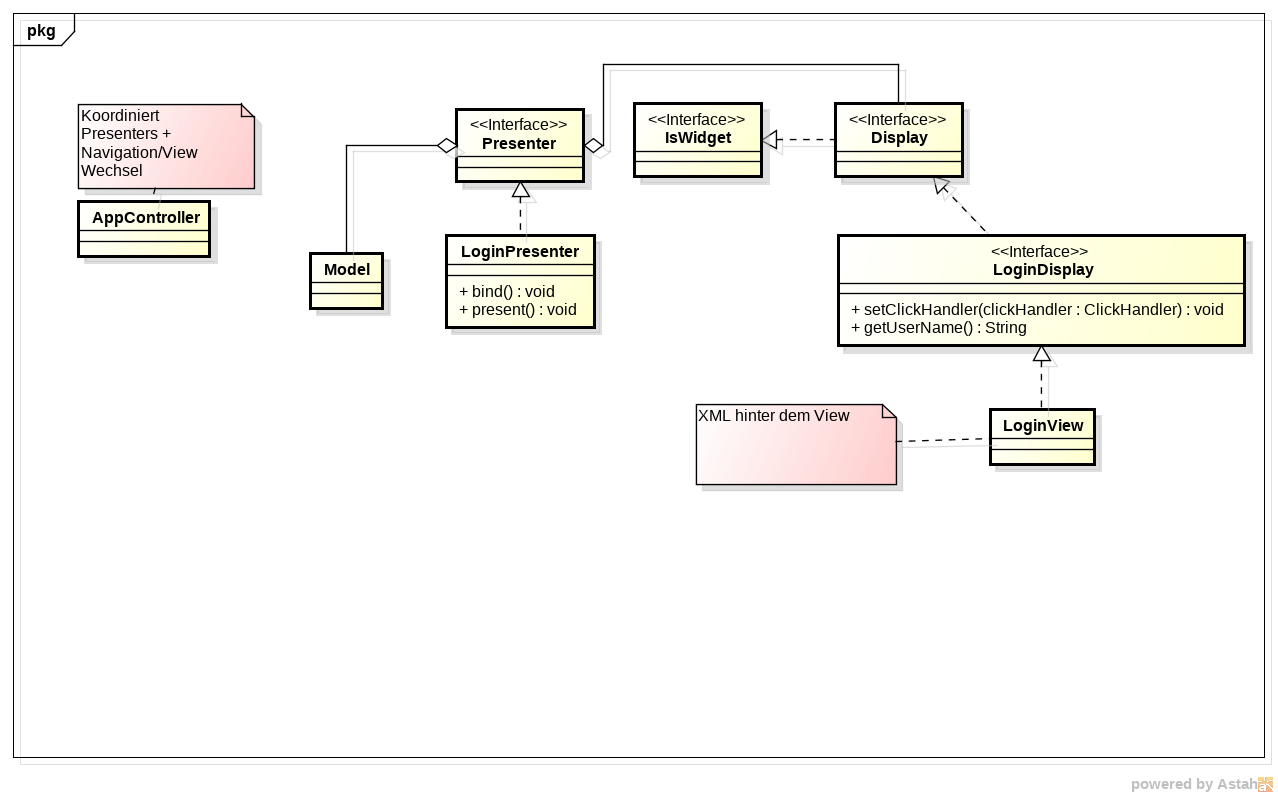
\includegraphics[scale=0.6,angle=90]{./wtextra.png}
 % wtextra.png: 1278x797 pixel, 96dpi, 33.81x21.08 cm, bb=0 0 958 598
\end{figure}

\textbf{Eventbus:}
\begin{itemize}
 \item Eventhandler System, ort wo sich Events hin und her schicken - Observer Pattern - register Listener.
 \item Weniger Koppleung zwischen App Controller und Presenter durch kommunikation mittels Events.
 \item Events kann auch an mehere interessierte Parteien gemeldet werden.
\end{itemize}

\chapter{History Management}

\section{Back Button Problem}
\begin{itemize}
 \item  Applikation mit GWT besteht nur aus eine Seite (Single Page - Hosting page)
 \item DOM Tree ständig verändert.
 \item Browser können nur ein Seitenwechsel zuverlässig detektieren. Browser können feststellen dass das DOM Tree sich 
verändert hat, aber können nicht der Grund der Veränderung feststellen (ob Navigation ist oder nicht z.B).
\item Browser History verändert sich deshalb nur bei Seitenwechsel.
\item Benutzer verlässt die Applikation dann ungewollt beim Klick auf dem Backbutton und verliert alle 
Zustandsinformationen. \textbf{Schwieriger History Management nachhinein einzubauen als von Anfgang an das dabei zu 
haben.}
\end{itemize}

\section{History Klasse}
GWT bietet dazu die Klasse com.google.gwt.user.client.History an, welche einfach
aber effizient Events des Back- und Forward-Buttons verarbeiten kann.
\subsection{URI Fragment als Token}
Die Methoden der History-Klasse sind statisch und erlauben einen Handler für die Back- und For-
ward-Buttons des Browsers zu registrieren. \underline{Um bei einer „Zeitreise“ mit Back oder Forward nicht
gleich die HTML-Seite zu verlassen, verwendet man den sogenannten URI Fragment Identifier.
Dies ist der Teil der URI nach einem Hashzeichen (\#). Für den Browser ist dies ein Ankerpunkt in
einer HTML-Seite. Er wird nicht die Seite neu laden, sondern nur zu diesem Anker springen. Und
genau dies macht sich das History-Management zunutze.}
Auf dem History-Stack werden sogenannte Tokens gespeichert. Ein Token ist der Text der URI
nach dem Hashzeichen. Es ist somit möglich jedem „zurückkehrbaren“ Zustand eine eindeutige
URI zuzuordnen und sogar noch mit Parametern zu versehen. Dieser Ansatz hat folgende Vorteile:
\begin{itemize}
 \item 1. Es ist die einzige zuverlässige Art die Browser-History zu kontrollieren
\item Der Entwickler behält die Kontrolle darüber, welche Zustände in die History aufgenom-
men werden.
\item Es ist „bookmarkable“, d.h. ein Zustand lässt sich als Bookmark bzw. als Favorit speichern.
\end{itemize}

\textbf{Bemerkungen:}
\begin{itemize}
 \item Die erwähnten Parameter können in beliebiger Form an das Token angehängt werden. Auf kei-
nen Fall dürfen Sie vor dem Hashzeichen stehen.
\item Hinter dem Token können
aber beliebig viele Parameter z.B. in der Form \texttt{?key1=value1\&key2=value2...} folgen. Es
gibt keine Vorschrift zum Format der Parameter, aber auch keine Unterstützung bei deren Erken-
nung. D.h. Parameter müssen selbst geparst werden.
\end{itemize}
\pic[Die History Klasse]{hc.png}

\section{Value Change Handler}
Wie kann ein Handler registriert werden, der aufgerufen wird, sobald sich die History ändert? Ein
com.google.gwt.event.logical.shared.ValueChangeHandler muss folgende
Methode implementieren:
\begin{lstlisting}
void onValueChange(ValueChangeEvent<T> event)
\end{lstlisting}
Wird nun die History geändert – sei es über die Back- und Forward-Buttons des Browsers, oder
programmatisch – so erhält man im Handler einen ValueChangedEvent<String>. Mit des-
sen getValue-Methode lässt sich das History-Token (inklusive eventueller Parameter) auslesen.
Als Typ-Parameter kann String verwendet werden, so ist kein Typcast bei der Verwendung der
getValue-Methode nötig:
\begin{lstlisting}
 public void onValueChange(ValueChangeEvent<String> event) {
String token = event.getValue();
// ...

//Die Klasse AppController bietet sich als zentraler Ort für die Verwaltung der Seitenübergänge an.
public class AppController implements Presenter, ValueChangeHandler<String> {
// ...
\end{lstlisting}
Warum sollte der AppController auch das Presenter Interface implementieren? Beim Aufstarten der
Applikation übernimmt der AppController ähnliche Aufgaben wie ein Presenter:
1. Er muss alle MVP-Patterns instanziieren und „verdrahten“
2. Er muss die Einstiegsseite anzeigen
Wie könnte also eine Implementation dieser MVP-Patterns zusammen mit dem AppController aussehen?
\begin{figure}[h]
 \centering
 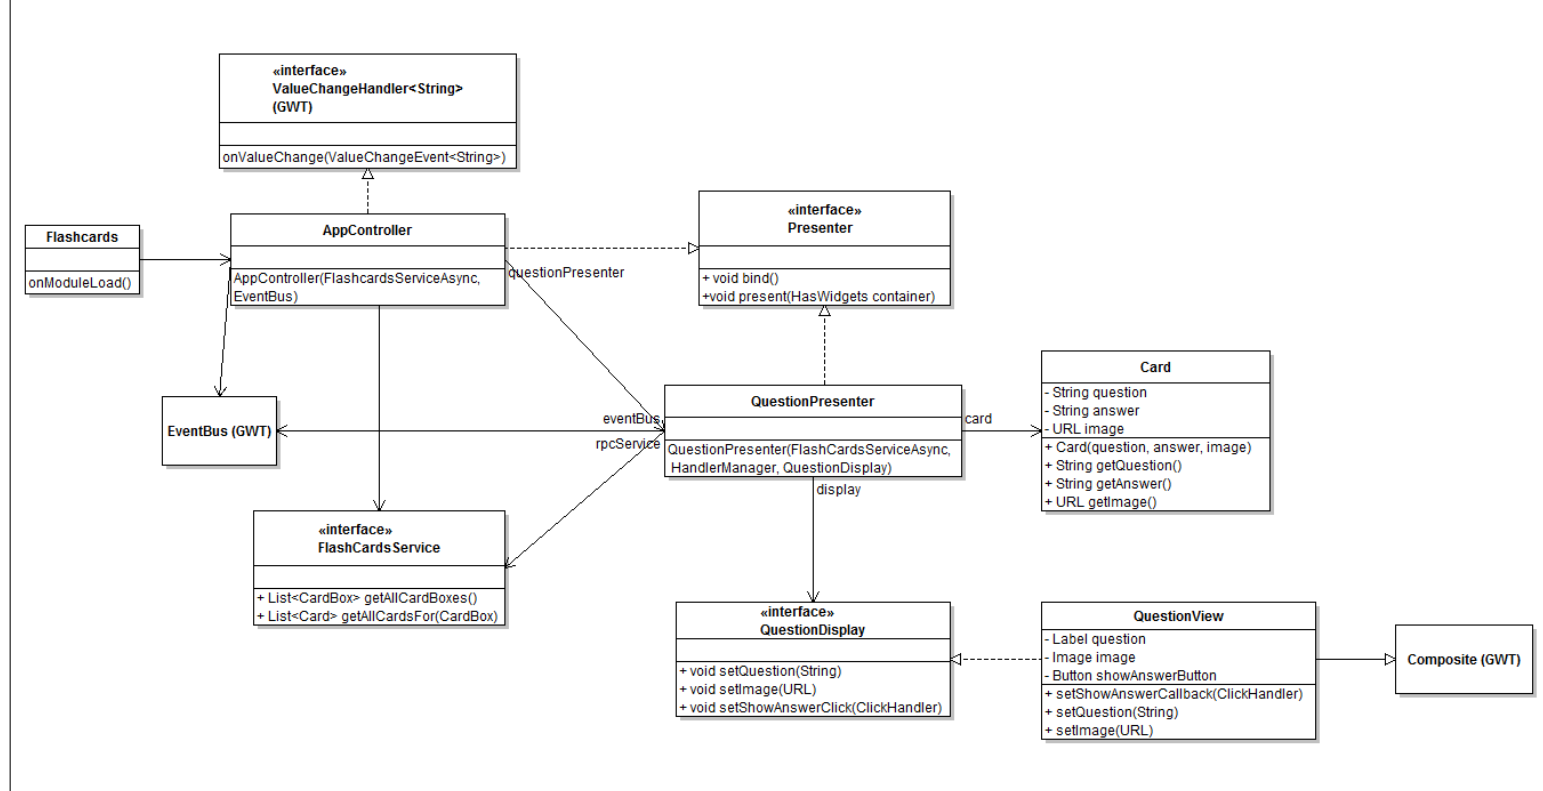
\includegraphics[angle=90,scale=0.5]{./apu1.png}
 % apu1.png: 1543x791 pixel, 72dpi, 54.43x27.90 cm, bb=0 0 1543 791
\end{figure}

\section{App Controller Code}

Konstruktor: \\
\begin{itemize}
 \item Initalisiert Eventbus
 \item Services initialisieren (rpc)
 \item Bind();
 \subitem Presenter erzugen und Initialisieren.
 \item Registriert sich als ValueChangeListener bei History Klasse
 \item Registriert Handler im Eventbus.
\end{itemize}

\begin{lstlisting}
 onValueChange(Event<string> event){
  String token = event.GetValue();
  Presenter p = null;
  if (token == null || "".equals(token||"start".equals(token)){
    p = WelconePresenter(rpcService,eventBus,new WelcomeView());
    }else if ("question".equals(token)){
    p = QuestionPresenter(eventBus,new QuestionView();}else if..
    
    if (p != null) {
     p.present(container);
    }
  }
 }
 
 //present methoden
 present(HasWidget container) {
 //immer noch im App Controller
 this.container == container;
 if ("".equals(Histroy.getToken()){
  History.newItem("welcome"); // feuert ValueChangeEvent
 }else {
  History.fireCurrentHistoryState();
 }
 }
\end{lstlisting}


\chapter{Kommunikation mit Server}
\section{Einführing - Erklärung von AJAX Request}
Die meisten JavaScript Engines in den Browsern sind single-threaded, d.h. sie können nicht mehrere
Aufgaben gleichzeitig (bzw. quasi-gleichzeitig) erledigen. Allerdings gibt es in JavaScript die Möglich-
keit http-Requests asynchron abzusetzen. Das bedeutet, dass der Request an den Server geschickt
wird und der Kontrollfluss unmittelbar danach wieder zum Aufrufer zurückkehrt, ohne dass eine
Antwort (Response) vom Server abgewartet wird. Kommt nun die http-Response vom Server zurück,
muss das Ergebnis irgendwie verarbeitet werden. Da das Ergebnis nicht wie ein Return-Wert zurück-
gegeben werden kann (der Kontrollfluss wartet das Ergebnis nicht ab) bleibt nur die Variante einen
zuvor installierten Callback-Handler aufzurufen.
\pic{ajax.png}

\subsection{Vorteile AJAX}
\begin{itemize}
 \item Ohne Ajax wird die Javascript Engine blokieren bis Resultät kommt. \textbf{Javascript ist singleThreaded}
 \item Server kann unnereichbar sein oder aus anderen Grunden nicht Antwoerten - Wie soll Client damit umgehen ohne 
ajax?
\item Ajax wird parallel zu Client Logik abgearbeitet, und Wartezeiten weden verkürtzt. (Beispiel : Rendering während 
wir auf Daten vom Server warten.)
\end{itemize}

\section{RPC - Remote Procedure Calls}
Für die Kommunikation mit einem Server bietet GWT – in Form von sogenannten Remote Procedure
Calls – eine sehr komfortable Unterstützung. Trotz des Namens unterscheiden sich RPC in GWT von
RPC in Unix oder RMI (Remote Method Invocation) in Java.
Der Hauptunterschied ist, dass Remote Procedure Calls in GWT immer asynchron ausgeführt werden.
Zudem sind RPCs immer nur in eine Richtung möglich, nämlich vom Client zum Server. Diese Ein-
schränkung ergibt sich durch die Verwendung des http-Protokolls für sämtliche Kommunikation zwi-
schen dem Browser und dem Server.
\subsection{RPC Pattern}
Serverseitig spricht man üblicherweise von Services, die gegenüber den Clients angeboten werden.
Ein Service ist ein Java-Interface, welches mehrere thematisch zusammengehörende Methoden ent-
hält.
Wie werden Services deklariert? Folgende Grafik soll eine Übersicht geben:
\pic{rpc.png}
Jeder Service wird durch eine kleine Gruppe an Hilfsinterfaces und -klassen implementiert. Auf der
Client-Seite müssen nur zwei Interfaces zur Verfügung gestellt werden damit ein Stub generiert wer-
den kann (in Form einer Proxy-Klasse). Der Stub ist für die Umwandlung des Methodenaufrufes in
einen Http-Request zuständig. Zudem wird im Stub der Request asynchron abgesetzt und auf eine
Server-Response gewartet. Diese Antwort wird dann wieder deserialisiert und in einen Methoden-
aufruf des zuvor registrierten Callbacks umgesetzt.
\subsection{RPC mit GWT}

Um ein Service-Interface zu definieren sind folgende Schritte nötig:
\begin{enumerate}
\item Definiere ein Java-Interface, das
com.google.gwt.user.client.rpc.RemoteService erweitert und alle benötig-
ten Service-Methoden enthält.
\item Implementiere eine Klasse, die den Server-seitigen Code enthält, von
com.google.gwt.user.server.rpc.RemoteServiceServlet abgeleitet ist und
das Interface von Punkt 1 implementiert.
\item Definiere ein asynchrones Interface zum Service, welches client-seitig aufgerufen werden
kann.
\end{enumerate}

\section{Namenskonventionen GWT RPC}
Um dem GWT-Compiler die korrekte Generierung von RPC-Code zu ermöglichen, ist es notwendig
einige Namenskonventionen einzuhalten. Dies betrifft vor allem die beiden Interfaces auf Clientseite:
\begin{itemize}
\item Ein Serviceinterface muss ein entsprechendes asynchrones Interface mit demselben Namen
und der Endung „Async“ haben. Zudem ist es notwendig, dass beide Interfaces im gleichen
Package deklariert werden. Beispiel: Ein Serviceinterface
ch.fhnw.webfr.client.FlashcardService muss ein asynchrones Interface
ch.fhnw.webfr.client.FlashcardServiceAsync haben.
\item Jede Methode im synchronen Interface muss eine entsprechende Methode im asynchronen
Interface mit einem zusätzlichen letzten Argument vom Typ
com.google.gwt.user.client.rpc.AsyncCallback<T> haben.
\end{itemize}

\section{Synchrone Interfaces mit GWT}
\begin{framed}
Das synchrone Interface spezifiziert den Service! Das asynchrone Interface muss sich danach richten.
Eine Implementation des Services auf Serverseite muss das synchrone Interface implementieren.
Wichtig: dieses Interface kann nicht direkt aufgerufen werden! Ein Aufruf muss über ein asynchrones
Interface erfolgen.
\end{framed}
\begin{lstlisting}
 package ch.fhnw.webfr.flashcards.client;
import java.util.List;
import com.google.gwt.user.client.rpc.RemoteService;
@RemoteServiceRelativePath("fcService")
public interface FlashcardsService extends RemoteService {
List<CardBoxInfo> getAllCardboxes(int minNofCards) throws IllegalArgumentException;
}
\end{lstlisting}

\section{Asynchrone Interface mit GWT}
Ein asynchrones Interface ist nötig, da alle RPCs asynchron abgesetzt werden. Ein asynchroner Aufruf
wird immer sofort zum Aufrufer zurückkehren und somit machen Return-Werte auch keinen Sinn.
Die Methoden in diesem Interface sind daher immer void. Um Ergebnisse aus dem Aufruf trotzdem
verarbeiten zu können, gibt es den Callback-Handler.
Das entsprechende asynchrone Interface muss demnach so aussehen:
\begin{lstlisting}
package ch.fhnw.webfr.flashcards.client;
import java.util.List;
import com.google.gwt.user.client.rpc.AsyncCallback;
public interface FlashcardsServiceAsync {
void getAllCardboxes(int minNofCards, AsyncCallback<List<CardBoxInfo>> callback);
}
\end{lstlisting}

\section{Callback Handlers}
Der Callback-Handler wird im asynchronen Interface als letztes Argument übergeben. Er steht anstel-
le eines Rückgabewertes und hat auch dessen Typ im Typparameter. Ein Callback-Handler wird auf
der Clientseite aufgerufen, sobald die Response vom Server beim Client ankommt. Ein Methodenauf-
ruf kann nur zwei Ergebnisse haben: Ein erwartetes Resultat oder einen Fehler (ein abnormes Ereig-
nis ist aufgetreten). Diese zwei Ergebnistypen werden durch die beiden Methoden des Typs
AsyncCallback<T> repräsentiert.
\begin{lstlisting}
 package com.google.gwt.user.client.rpc;
public interface AsyncCallback<T> {
void onFailure(java.lang.Throwable caught);
void onSuccess(T result);
}
\end{lstlisting}

Der Typparameter <T> entspricht dem Return-Typ der Methode im synchronen Interface.
Die onSuccess-Methode erhält als einziges Argument das Resultat des Methodenaufrufes. Sie wird
im Falle einer normalen Ausführung der Methode aufgerufen.
Die onFailure-Methode wird immer dann aufgerufen, wenn in der Methode selbst eine Exception
geworfen wurde oder wenn es Probleme mit dem Aufruf oder der Antwort bzw. deren Übermittlung
gab (z.B. Timeout).

\section{Implementation der Interface}
Die Implementation der Servicemethoden erfolgt in einer Server-Klasse, die gleichzeitig auch ein
Servlet ist. Dazu wird die Klasse RemoteServiceServlet erweitert und das synchrone Interface
implementiert:
\begin{lstlisting}
 package ch.fhnw.webfr.flashcards.server;
// import statements here
public class FlashcardsServiceImpl extends RemoteServiceServlet
implements FlashcardsService {
@Override
public List<CardBoxInfo> getAllCardboxes(int minNofCards) throws IllegalArgumentException
{
return new LinkedList<CardBoxInfo>();
}
}
\end{lstlisting}
Die Basisklasse RemoteServiceServlet kümmert sich um die Deserialisierung der Argumente
(http-Request) und die Serialisierung (http-Response) der Return-Werte. In den meisten Fällen hat
der Entwickler nichts mit diesen oder anderen Servletmethoden zu tun.

\section{Parameter und Ruckgabetypen}
Sämtliche Argumente sowie die Rückgabewerte müssen über das Netzwerk vom Browser zum Server
und zurück. Dies bedeutet, dass alle Argumente und Rückgabewerte serialisierbar sein müssen. Auf
folgende Punkte ist zu achten:
\begin{itemize}
 \item Alle Klassen die als Parameter oder Rückgabetypen verwendet werden, müssen
java.io.Serializable implementieren.
\item Alle Klassen die als Parameter oder Rückgabetypen verwendet werden, müssen einen
Default-Konstruktor (d.h. einen Konstruktor ohne Argumente) oder gar keinen Konstruktor
haben.
\item Falls Collections verwendet werden, sollte unbedingt der Typ der Elemente angegeben
werden, also z.B. List<CardBoxInfo>. Die Verwendung von rohen Typen oder von
Object funktioniert nicht, da java.lang.Object selbst nicht Serializable ist.
\end{itemize}

\section{RPC Aufruf Prozess von Client aus}
\begin{lstlisting}
 public void makeCall() {
// (1) create a stub object that implements the asynchronous interface.
FlashcardsServiceAsync service = GWT.create(FlashcardsService.class);
// (2) Define a callback handler.
AsyncCallback<List<CardBoxInfo>> callback = new AsyncCallback<List<CardBoxInfo>>() {
@Override
public void onFailure(Throwable caught) {
// do some stuff on failure.
}
@Override
public void onSuccess(List<CardBoxInfo> result) {
// use result for further processing.
}
};
// (3) make the call.
service.getAllCardboxes(0, callback);
// remember this call was asynchronous! Control flow will continue
// immediately here.
nextStatement();
}
\end{lstlisting}
\begin{enumerate}
 \item Zuerst muss der Service mittels GWT.create()instanziiert werden.
\item Dann muss ein asynchrones Callback-Objekt erzeugt werden, welches benachrichtigt wird,
wenn der RPC beendet ist.
\item Den Aufruf über das asynchrone Interface machen.
\end{enumerate}

\section{Serveradresse für Aufrufe}
\pic{serveradrrpc.png}
\begin{lstlisting}[caption=RPC App Deployment Descriptor,language=xml]
 <servlet>
<servlet-name>cardsServlet</servlet-name>
<servlet-class>
ch.fhnw.webfr.flashcards.server.FlashcardsServiceImpl
</servlet-class>
</servlet>
<servlet-mapping>
<servlet-name>cardsServlet</servlet-name>
<url-pattern>/flashcards/fcService</url-pattern>
</servlet-mapping>
\end{lstlisting}
Der Kontextpfad /flashcards im URL-Pattern muss mit dem Namen der Applikation im Konfigu-
rationsfile Flashcards.gwt.xml in der Moduldeklaration vermerkt sein

\chapter{Deployment}
Das Laden einer Webapplikation geschieht immer wenn ein/e Benutzer/-in wartet. Zudem wird die
Applikation über das Internet und nicht von lokalen Datenträgern geladen. Um lange Wartezeiten zu
vermeiden versucht man bei grösseren Applikationen diese in mehreren Schritten zu laden und zwar
nur dann wenn die einzelnen Teile auch wirklich gebraucht werden.

\section{Defered Binding}
Der GWT-Compiler erzeugt immer ein .war-File, das neben den Javascript-Files auch die Java-Class-
Files (für den Server) sowie auch alle nötigen Ressourcen (Bilder, Icons, Audio- und Video, etc.) ent-
hält. Der Compilationsvorgang in GWT ist nicht nur deswegen aufwändiger und langsamer als der von
normalen Java-Applikationen. Denn zusätzlich werden mehrere Compilate erstellt für verschiedene
Browsertypen und verschiedene Locales.
\begin{figure}[h]
 \centering
 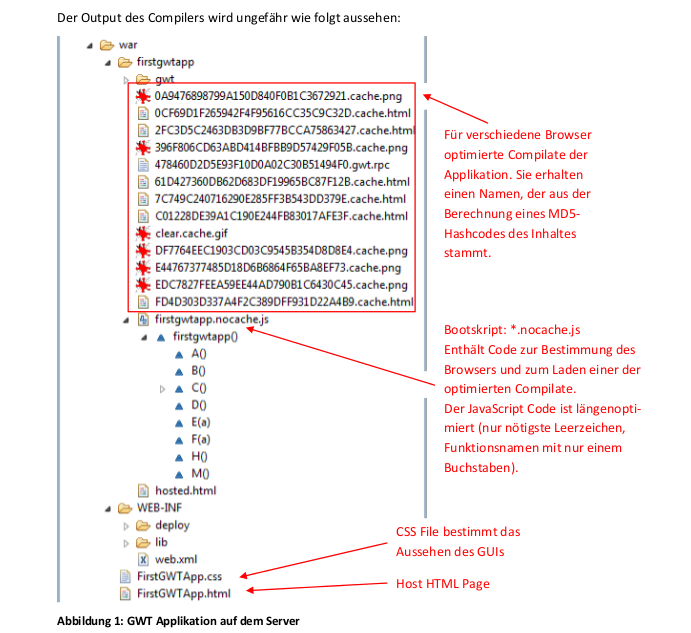
\includegraphics[scale=0.6]{./dbind.png}
 % dbind.png: 691x633 pixel, 72dpi, 24.38x22.33 cm, bb=0 0 691 633
\end{figure}
\begin{lstlisting}[caption=GWT Einstiegsseite,language=html]
 html>
<head>
<meta http-equiv="content-type" content="text/html; charset=UTF-8">
<link type="text/css" rel="stylesheet" href=" FirstGWTApp.css">
<title>First GWT Application</title>
<script type="text/javascript" src='firstgwtapp/firstgwtapp.nocache.js'/>
</head>
<body>
<noscript><div>Please enable JavaScript</div></noscript>
<!-- more body content here.
-->
</body>
</html>
\end{lstlisting}
Das angegebene Skriptfile wird geladen und ausgeführt. In diesem Bootskript wird der aktuelle
Browser und dessen Version, sowie das eingestellte Locale bestimmt. Danach wird das dazu passen-
de <md5>.cache.html nachgeladen. Dieses ist eines der optimierten Compilate.
Eine detaillierte Beschreibung dieses Bootstrap-Prozesses findet sich hier:
\texttt{http://code.google.com/webtoolkit/doc/latest/DevGuideOrganizingProjects.html\#DevGuideBootstrap}

Die Namensgebung ist nicht zufällig und erlaubt das Caching der Seiten zu optimieren. Bei jeder
Compilation werden neue MD5-Hashcodes berechnet und die Applikationsfiles danach benannt.
Wichtig ist nun, dass das *.nocache.js-File ein sofortiges Verfallsdatum erhält. D.h. der Webser-
ver sollte diesen Files eine Gültigkeitsdauer von 0 Sekunden geben (<meta http-
equiv="expires" content="0"> im HTML-HEAD-Tag), damit die Browser das Bootskript nicht
im Cache behalten. Bei jedem Anwählen der Applikation wird nun das *.nocache.js Skript neu
geladen. Falls sich nichts geändert hat, wird im Browser die lokal gecachte Applikationsdatei ausge-
führt (die verfällt z.B. innerhalb eines Jahres). Bei einer Änderung wird aber das Applikationsfile ei-
nen neuen MD5-Code und damit einen neuen Namen erhalten. Der Browser wird es somit nicht im
Cache finden und automatisch die aktuelle Version herunterladen und ausführen. Dies ist vor allem
beim Debugging sehr praktisch, da keine Caches geleert oder Browser neu gestartet werden müssen.
Ein Reload der Seite genügt.
Dieser Vorgang des Ladens einer Applikation nennt sich Deferred Binding.

\section{Compilation}
Der GWT Compiler erstellt pro Browserfamilie und Locale jeweils ein Compilat. Es enthält den gesam-
ten Applikationscode ohne unnötige Leerzeichen und mit möglichst kurzen Bezeichnernamen. Zudem
enthält es auch alle für das eingestellte Locale relevanten Texte und Medienfiles. Damit werden
gleich drei Anforderungen auf einmal erfüllt:
\begin{enumerate}
\item Die Ladezeit wird verkürzt weil die Files kleiner sind.
\item Der Code wird kleiner, weil keine unnötigen Übersetzungen und (übersetzte) Medienfiles
übertragen werden müssen.
\item Der Code läuft schneller, weil Fallunterscheidungen entfallen.
\end{enumerate}
Die Abbildung 2 zeigt in welcher Reihenfolge diese Compilate erstellt werden.
Während der Entwicklung sollte immer wieder mal eine Compilation durchgeführt werden um mög-
lichst früh herauszufinden, ob keine zur JRE Emulation inkompatiblen Sprachkonstrukte oder Biblio-
theksmodule verwendet wurden.

\pic[Compilate Matrix]{cpm.png}
\newpage
\begin{lstlisting}[language={}]
 Falls der Code so schnell wie möglich compiliert werden soll, dann sollten folgende Optionen in Be-
tracht gezogen werden um Optimierunen auszuschalten:
-draftCompile –optimize 0
Zudem sollte im .gwt.xml File noch folgende Zeilen eingefügt werden damit nur eine Codeversion
produziert wird:
<set-property name="user.agent" value="gecko"/>
<set-property name="locale" value="en" />
Andererseits bieten die Optionen
-XdisableCastChecking –XdisableClassMetadata -style OBF
eine gute Ausgangslage für möglichst kompakten Code, so wie man ihn für die Release-Version ha-
ben will. Die wenigen dokumentierten Compileroptionen sind unter folgendem Link zu finden:
http://code.google.com/webtoolkit/doc/latest/DevGuideCompilingAndDebugging.html#DevGuideCompilerOptions.
\end{lstlisting}

\section{Code Splitting}
  Wenn eine Applikation grösser wird (man beachte den Gebrauch von wenn anstelle von falls :-) kann
der initiale Download zu spürbaren Wartezeiten führen. Um dies zu verhindern kann eine Applikation
beim Starten vorerst nur einen Teil laden. Danach werden dann bei Bedarf oder im Hintergrund all-
mählich weitere Teile nachgeladen.
Was ist der Unterschied zum Deferred Binding?
\begin{itemize}
\item Der Applikationsprogrammierer /-designer legt explizit fest, wo das Code Splitting zum Einsatz
kommt, das Deferred Binding ist eine GWT Optimierung die automatisch erzeugt wird.

\item Code Splitting teilt die gesamte Applikation in mehrere Teile auf während Deferred Binding die
Aufteilung gemäss Browserfamilien vornimmt.
\end{itemize}

Code Splitting ist eine oft verwendete Technik auch in herkömmlichen Ajax Applikationen um die
Wartezeit beim Aufstarten einer Applikation zu verringern. Code Splitting kann auf zwei verschiedene
Arten eingesetzt werden. Dabei wird immer zuerst ein erster Teil der Applikation geladen, z.B. eine
Welcome-View die dem Benutzer mehrere Optionen bietet. Danach kann wie folgt fortgefahren
werden:
\begin{itemize}
\item Während der User noch über seine Möglichkeiten nachdenkt oder erste Eingaben auf der Wel-
come-View macht, wird im Hintergrund (asynchron!) der Rest der Applikation geladen.
Mit diesem Ansatz wird die Zeit bis die komplette Applikation im Browser ist zwar objektiv ver-
längert (das Laden von mehreren Code-Paketen ist immer langsamer als das Laden eines einzigen
Paketes). Subjektiv nimmt der Benutzer diese Wartezeit aber nicht wahr, da er z.B. mit der Ein-
gabe seines Passwortes beschäftigt ist.
\item Die weiteren Teile der Applikation werden erst bei Bedarf geladen, also erst dann wenn der Be-
nutzer z.B. darauf klickt. Im Gegensatz zum ersten Ansatz wird hier Speicher und Bandbreite ge-
spart, da nur diese Teile der Applikation heruntergeladen werden, die auch tatsächlich benötigt
werden. Allerdings kann es so immer wieder zu Wartezeiten kommen. Beispiel zur Lernkartei
(Flashcards): wenn nur gelernt wird, braucht es kein Code zum Editieren von Karten.

\end{itemize}
Die Kosten für einen Codesplit müssen nur einmal bezahlt werden: Wenn ein Teil der Applikation
einmal heruntergeladen wurde, dann wird er nicht ein weiteres Mal beim Server angefordert.

\chapter{Testing}

\section{Herkömmliche Ajax Apps}
Testen von herkömmlichen RIAs ist sehr aufwändig da deren client-seitiger Code in Javascript entwi-
ckelt wurde. Um diesen Javascript-Code zu testen muss eine Javascript Engine zur Verfügung stehen.
Alle Tests müssen zuerst auf die JS-Engine deployed werden, bevor sie ausgeführt werden können.
Daraus ergeben sich folgende Probleme:
\begin{itemize}
\item Lässt sich ein Test oder eine Testsuite automatisiert (z.B. mit Ant) deployen?
\item Ist die JS-Engine in der Lage verschiedene Browser zu simulieren?
\item Ist es möglich die verschiedenen Browser z.B. mittels Plugins zu erweitern, so dass ein auto-
matisiertes Deployment durchführbar ist. Sind die Schnittstellen für solche Plugins auf den
unterschiedlichen Browsern wenigstens einheitlich ansprechbar?
\item Stehen vernünftige Debugger für die JS-Engine zur Verfügung? D.h. kann der Code schrittwei-
se durchlaufen und können Variableninhalte inspiziert werden?
\item Werden .js-Files unterstützt? Oder müssen Tests in html-Files verpackt werden?
\item Kann dasselbe Testing-Framework sowohl Server- als auch Client-seitig verwendet werden?
\item Stehen Testing Tools wie Mock-Frameworks, Code-Coverage oder Metrik-Tools zur Verfü-
gung? Auf allen wichtigen Browsern? Mit gleichen Schnittstellen, damit automatisiert getes-
tet werden kann?

\end{itemize}
Leider müssen oft gleich mehrere dieser Fragen mit „Nein“ beantwortet werden. Das Testen von JS-
Code wird so zu einer sehr mühsamen Angelegenheit, die aufwändig zu implementieren und durch-
zuführen ist. Als Konsequenz wird dann häufig auf Tests verzichtet, gerade mit dem Hinweis auf die
hohen zusätzlichen Aufwände.

\section{GWT Testing}
Ganz anders sieht es für GWT-Applikationen aus: da der grösste Teil der Entwicklung in Java erfolgt,
können zu grossen Teilen auch die gewohnten Java Testing Tools zum Einsatz kommen:
\begin{itemize}
 \item JUnit als Basisframework – es wird nicht nur für Unit-Tests eingesetzt, sondern dient häufig
auch als Treiberplattform für Integrations- oder GUI-Tests.
EasyMock, Mockito, jMock, etc.
\item Code Coverage mit Emma, Cobertura, etc.
\item Bug-Finder und Stylechecker wie Checkstyle, Findbugs, PMD
\item Und viele andere Tools, die häufig dann auch noch aus der gewohnten Entwicklungsumge-
bung wie Eclipse, Netbeans oder IntelliJ verwendet werden können (im Gegensatz zu Brow-
serplugins)
\end{itemize}
Doch es ist nicht alles mit Java und den gewohnten Tools machbar. Einige Einschränkungen existie-
ren:
\begin{itemize}
 \item Tests von Klassen oder Komponenten, die GWT-Libraries verwenden (diese stehen in J2SE-
Umgebungen nicht zur Verfügung), insbesondere GUI-Tests!
\item Test der Kommunikation zwischen Client und Server
\item Tests von Servlets (serverseitiger Code) die einen Servlet-Container (z.B. Tomcat) benötigen.
\end{itemize}

\section{Vorbereitung Arch und Design}
Eine gute Planung der Architektur einer GWT-Applikation hilft enorm dabei, möglichst viel Code mit
Unittests zu versehen. Zwei Entwurfsmuster sind dabei besonders hervorzuheben:

\begin{enumerate}
\item Das MVP-Pattern hilft Verantwortlichkeiten aufzutrennen. Das Modell kann meist vollständig
in Plain Java entwickelt werden, ohne zusätzliche Unterstützung durch GWT-Libraries oder
Servlet-Container. Der Presenter kann zu einem grossen Teil auch komplett in Plain Java
entwickelt werden. Dazu ist es nötig eine klare Trennung von der View mittels Display-
Interfaces vorzunehmen. Dadurch kann die View mit Mock-Objekten „simuliert“ werden und
es sind keine GWT-Libraries notwendig.
\item Dependency-Injection unterstützt das oben erwähnte Mocking. Als Beispiel: ein Presenter er-
zeugt nicht selbst eine View, sondern erhält diese mittels einem Display-Argument über ei-
nen Setter oder direkt in den Konstruktor.
\end{enumerate}
Weitere Entwurfsmuster wie Factories, State-/Strategy-Pattern oder Decorators helfen Objekte un-
abhängig von ihrem konkreten Typ zu erstellen, zu verwalten oder einzusetzen.

Wenn die Architektur einer GWT-Applikation zum vornherein die gängigen Entwurfsprinzipien ein-
hält ist also ein sehr grosser Teil der Applikation mit herkömmlichen Mitteln testbar. Wie steht es
aber mit dem Rest der Applikation, der nicht ohne GWT-Libraries oder Servlet-Container auskommt?

\section{GWTTestCase}
GWT verwendet HTMLUnit als eingebauter Browser und da HTMLUnit in Java geschrieben ist, ist es
möglich Tests im Development-Mode zu debuggen. In Integrationstests ist es sogar möglich Klassen
die Javascript verwenden zu testen.
Allerdings gibt es auch Nachteile: Da es zwischen dem Development-Mode und dem Production-
Mode subtile Unterschiede gibt (z.B. die unvollständige JRE-Emulation), können nicht alle Probleme
mit GWTTestCase erkannt werden. Zudem ist es nicht möglich Mocking-Frameworks wie EasyMock
einzusetzen (weil diese Reflection verwenden, was in der JRE-Emulation nicht unterstützt wird).
\section{Selenium}
Selenium ist ein Testwerkzeug für Webapplikationen, das sich vor allem für Akzeptanztests gut eig-
net. Mit dem Firefox Plugin Selenium IDE kann im Browser eine Eingabesequenz aufgezeichnet und
danach in einem einfachen Editor bearbeitet werden. Die aufgezeichneten Skripts können dann –
auch automatisiert – wieder abgespielt werden. Da Selenium völlig unabhängig von GWT ist, kann es
für beliebige Web-Frameworks als Akzeptanztesttool verwendet werden. Der Einsatz von Selenium
sollte mit Vorteil erst dann erfolgen, wenn das GUI einigermassen stabil ist und kaum noch Änderun-
gen zu erwarten sind. Die Kombination von GWT und Selenium ist eher aufwändig, da zur eindeuti-
gen Identifikation von Widgets deren IDs verwendet werden. Leider können die IDs nicht mit dem
UIBuilder zugewiesen werden und müssen daher mühsam von Hand im Code gesetzt werden.
\chapter{HTML 5}
\section{Motivation}
Dynamische Websites sind Standard,
Interaktionen zwischen Usern (Mail, Facebook ,Twitter, etc) sowie schnell reagierende Rich
Internet Applications gehören zum guten Ton. Nicht zu vergessen sind Anforderungen an die
Sicherheit aber auch an die Barrierefreiheit von Websites.

\section{Features}
HTML5 will in einigen Bereichen HTML an heutige Bedürfnisse anpassen.
\begin{itemize}
 \item Neue Input-Elemente wie
\subitem Sliders <input type="range">
\subitem Color Pickers <input type="color">
\subitem Telefonnummern <input type="tel">
\subitem Adressen <input type="email">
\subitem Kalender-Date Pickers <input type="date">
\subitem und einige mehr...
\item Placeholder Texte sind Texte, die in einem Textfeld angezeigt werden, bevor die Benutzerin
zum ersten Mal etwas hineinschreibt. Sie können verwendet werden um Hinweise zu geben,
was das Eingabefeld erwartet.
\item  Autofocus setzt den Cursor beim Anzeigen einer Seite automatisch in ein bestimmtes
Inputfeld.
\item  Geolocation: ein API das es ermöglicht, den Standort des Browsers zu bestimmen.
\item  Web Workers: das ist ein Standard um Javascript im Hintergrund auszuführen, bzw. mehrere
Threads zu starten.
\item  Offline-Applikationen: Ermöglicht es Webapplikationen auch zu funktionieren, wenn der
Browser offline ist.
\item  Lokaler Speicher: Dem Web-Entwickler steht (mehr oder weniger beschränkt) lokaler
Speicher zur Verfügung um Daten auf dem Client zu speichern. Nützlich auch im
Zusammenhang mit Offline-Fähigkeit.
\subitem  Video: Anzeige von Audio und Video-Dateien ohne Plugins
\subitem  Canvas: eine Fläche die beliebig „bemalt“ werden kann.
\subitem Semantische Elemente wie <section>, <article>, <nav>, <footer>... Sie
helfen den Text inhaltlich zu strukturieren.
\item  Microdata: eine Möglichkeit den DOM-Baum semantisch zu annotieren und damit auch ein
Schritt in Richtung „semantic web“.
\end{itemize}

Ist das alles? Ja! Was soll daran neu sein? Ausser dem Standard – nichts. Aber das ist schon eine
ganze Menge! Viele der bisherigen Lösungen der oben beschriebenen Features beruhten auf
Plugins, umfangreichen Javascript-Libraries oder schlicht auf Hacks. Ein Standard vereinfacht
diese Situation
\begin{itemize}
 \item Features wie Video, lokaler Speicher oder Offline-Support sind nun auf allen HTML5-fähigen
Browsern vorhanden, auch dort wo (z.B. aus Sicherheitsgründen) keine Plugins installiert
sind.
\item Features wie Placeholder Texte und Autofocus sind einheitlich gelöst und müssen nicht für
jede Website neu implementiert werden. Gerade das Autofocus-Feature war immer eine
mühsame Fallunterscheidung zwischen den verschiedenen Browsertypen um die
Eventreihenfolge richtig zu implementieren.
\item Die neuen Input-Elemente vereinfachen in vielen Fällen die Validierung der Benutzereingabe.
Gerade Email-Adressen entpuppen sich als erstaunlich komplex (siehe z.B.
http://www.regular-expressions.info/email.html )
\item Zudem ist es nicht mehr nötig diesen Code für jede Website neu als JS-Bibliothek
herunterzuladen. Der Code ist im Browser, dort geht er nicht vergessen und ist
wahrscheinlich stabiler als stetig wiederholter Skriptcode.
\end{itemize}

\section{Mobile Geräte}
Viele der Neuerungen sind für herkömmliche Webbrowser tatsächlich nicht atemberaubend.
Interessant ist HTML5 allerdings auch für die mobilen Geräte! So unterstützt iPhone viele HTML5
Features, webOS von HP/Palm baut sogar auf Javascript und HTML5 als Basis für die
Applikationsentwicklung. Wo liegen die Vorteile für mobile Geräte?
\begin{itemize}
\item Mobile Geräte haben oft eine langsamere Verbindung ins Internet. Benutzer sind dankbar
für jede JS-Library die nicht heruntergeladen werden muss.
\item Verbindungen können unterwegs immer mal wieder abreissen (z.B. in Tunnels). Da ist man
froh um lokalen (Zwischen-)Speicher und Offline-Funktionalitäten.
\item Geolocations machen auf einem stationären PC der seine IP-Nummer über einen (weit
entfernten) Provider bezieht nicht wirklich Sinn.
\item Plugins sind für mobile Geräte auch oft ein Tabu – einerseits aus Sicherheitsgründen,
andererseits auch wegen der beschränkten Anzeigefläche.
\item Die neuen Inputelemente bieten nicht nur eine Validierung an, sondern sie geben dem
mobilen Gerät auch einen Hinweis welche Tastatur eingeblendet werden soll. Wird also eine
Telefonnummer verlangt, kann das iPhone z.B. eine Tastatur verwenden, die nur Ziffern, *, \#
und + aufweist.
\end{itemize}

\section{Chaos mit Standards}
Nein! Das Durcheinander von „Standards“ wird auch in Zukunft bleiben, ja sich vielleicht sogar
noch verschärfen, da jetzt auch die mobilen Browser mitmischen werden. Gründe warum es auf
absehbare Zeit nicht einfacher werden wird mit HTML umzugehen:
\begin{itemize}
 \item Rückwärtkompatibilität HTML 5
 \item Kein Standard - W3C Working Draft.
 \item Es stehen handfeste Interessen hinter den Produkten. Jeder Browserhersteller möchte sich
so gut wie möglich positionieren und den anderen so wenige Chancen wie möglich bieten,
eine bessere Position zu erlangen. Als Beispiel hierfür kann der lokale Speicher genommen
werden. Es gab Bestrebungen eine Datenbank in die Browser zu integrieren, damit nicht nur
Key-Value-Paare persistent gespeichert werden können. Die sogenannte WebDB lehnte sich
stark an SQLLite an. So stark, dass man nicht mehr von einem offenen Standard sprechen
kann (was die Spezifikation selbst sogar zugibt). Mozilla und Microsoft haben WebDB nicht
übernommen.
\end{itemize}
\part{Arbeitsblätter,Übungen,Code}
\chapter{MVP, Navigation}
\lstinputlisting[caption=EntryPoint]{umvp/mvp1.java}
\lstinputlisting[caption=AppController]{umvp/mvp2.java}
\lstinputlisting[caption=OneView]{umvp/mvp3.java}
\lstinputlisting[caption=WelcomeView]{umvp/mvp4.java}
\begin{lstlisting}[caption=WelcomeView xml,language=xml]
 <!DOCTYPE ui:UiBinder SYSTEM "http://dl.google.com/gwt/DTD/xhtml.ent">
<ui:UiBinder xmlns:ui="urn:ui:com.google.gwt.uibinder"
	xmlns:g="urn:import:com.google.gwt.user.client.ui">
	<ui:style>
		.important {
			font-weight: bold;
		}
	</ui:style>
	<g:HTMLPanel>
		<g:Button styleName="{style.important}" ui:field="one" />
		<g:Button styleName="{style.important}" ui:field="two" />
	</g:HTMLPanel>
</ui:UiBinder> 
\end{lstlisting}

\lstinputlisting[caption=WelcomePresenter]{umvp/mvp5.java}
\lstinputlisting[caption=OnePresenter]{umvp/mvp6.java}
\chapter{History Management}
\lstinputlisting[caption=App Controller]{uhm/appc.java}
\lstinputlisting[caption=OneView]{uhm/OneView.java}
\lstinputlisting[caption=WelcomeView]{uhm/WelcomeView.java}
\lstinputlisting[caption=WelcomePresenter]{uhm/WelcomePresenter.java}
\lstinputlisting[caption=OnePresenter]{uhm/OnePresenter.java}
\lstinputlisting[caption=IncEvent]{uhm/IncEvent.java}
\lstinputlisting[caption=IncEventHandler]{uhm/IncEventHandler.java}
\chapter{RPC}
\section{Client}
\lstinputlisting[caption=Entry Point]{urpc/client/SearchAsYouType.java}
\lstinputlisting[caption=Search as You Type Service]{urpc/client/SaytService.java}
\lstinputlisting[caption=Search as You Type Service Async]{urpc/client/SaytServiceAsync.java}
\lstinputlisting[caption=Search Panel]{urpc/client/SearchPanel.java}
\begin{lstlisting}[caption=search panel xhtml,language=xml]
 <!DOCTYPE ui:UiBinder SYSTEM "http://dl.google.com/gwt/DTD/xhtml.ent">
<ui:UiBinder xmlns:ui="urn:ui:com.google.gwt.uibinder"
	xmlns:g="urn:import:com.google.gwt.user.client.ui" xmlns:p1="urn:import:com.google.gwt.user.cellview.client">
	<g:HTMLPanel>
		<g:VerticalPanel>
			<g:Label text="Bitte Suchtext eingeben:"/>
			<g:TextBox alignment="LEFT" visibleLength="50" ui:field="textBox"/>
			<g:Label text="Resultate:"/>
			<p1:CellList ui:field="addressList"/>
		</g:VerticalPanel>
	</g:HTMLPanel>
</ui:UiBinder> 
\end{lstlisting}

\section{Server}
\lstinputlisting[caption=AddressProvider]{urpc/server/AddressProvider.java}
\lstinputlisting[caption=SaytServiceImpl]{urpc/server/SaytServiceImpl.java}

\section{Shared}
\begin{lstlisting}
 package ch.fhnw.webfr.sayt.shared;

import java.io.Serializable;

/**
 * Data container for a Swiss address.
 * @author Christoph Denzler
 *
 */
public class Address implements Serializable {
	private String lastname;
	private String firstname;
	private String street;
	private int streetnr;
	private int plz;	
	private String city;	
	
	public Address(String firstname, String lastname, String street, int streetnr, int plz, String city) {
		this.firstname = firstname;
		this.lastname = lastname;
		this.street = street;
		this.streetnr = streetnr;
		this.plz = plz;
		this.city = city;		
	}
	
	public Address() {
	}
	
	
	public String getLastname() {
		return lastname;
	}


	public String getFirstname() {
		return firstname;
	}


	public String getStreet() {
		return street;
	}


	public int getStreetnr() {
		return streetnr;
	}


	public int getPlz() {
		return plz;
	}


	public String getCity() {
		return city;
	}

}
\end{lstlisting}

\end{document}